\subsection{Wikidata}
Wikidata is the free and open database by the Wikimedia movement. Similar to the Wikipedia it is user editable. Wikidata collects data on different topics like people, places, events and many more. Due to the structure of Wikidata, the data is multilingual.
\begin{figure}[ht]
	\centering
	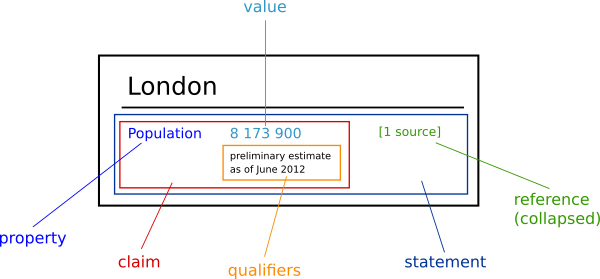
\includegraphics[width=120mm]{diagrams/Wikidata_statement.png}
	\caption{Wikidata Statement for item London}
	\label{fig1}
\end{figure}

Every item has a unique identifier, starting with a ``Q''. Therefore it is clearly identifiable and not depending on labels, which may change. \\
Statements contain a property, which is the core part and indicating, what kind of statement is made. One or more values are attached to this property. For example, a statement for a city could be number of inhabitants. There can be multiple values for population of multiple years, differentiated by qualifiers. To identify the important and most recent data, the values can be ordered as preferred, normal and deprecated rank.\\
Data types for the other items are other items, string, quantity, names of Wikimedia Commons files, geo coordinate, time, URL,  and in the future also identifier of other databases like VIAF. \\
The data is under a CC-0 licence and therefore free to anyone to copy, use and distribute.
The aim is not only to have a database that supports the Wikipedia but can also be used in other contexts in the semantic web. Therefore, Wikidata offers an API as well as an SPARQL endpoint. Additionally, the data can be downloaded as a full database dump in the formats JSON, XML and RDF.  